% !TEX root = ../00_tcc.tex

\begin{figure}[H]
	\centering
	\begin{subfigure}[b]{\textwidth}
		\centering
		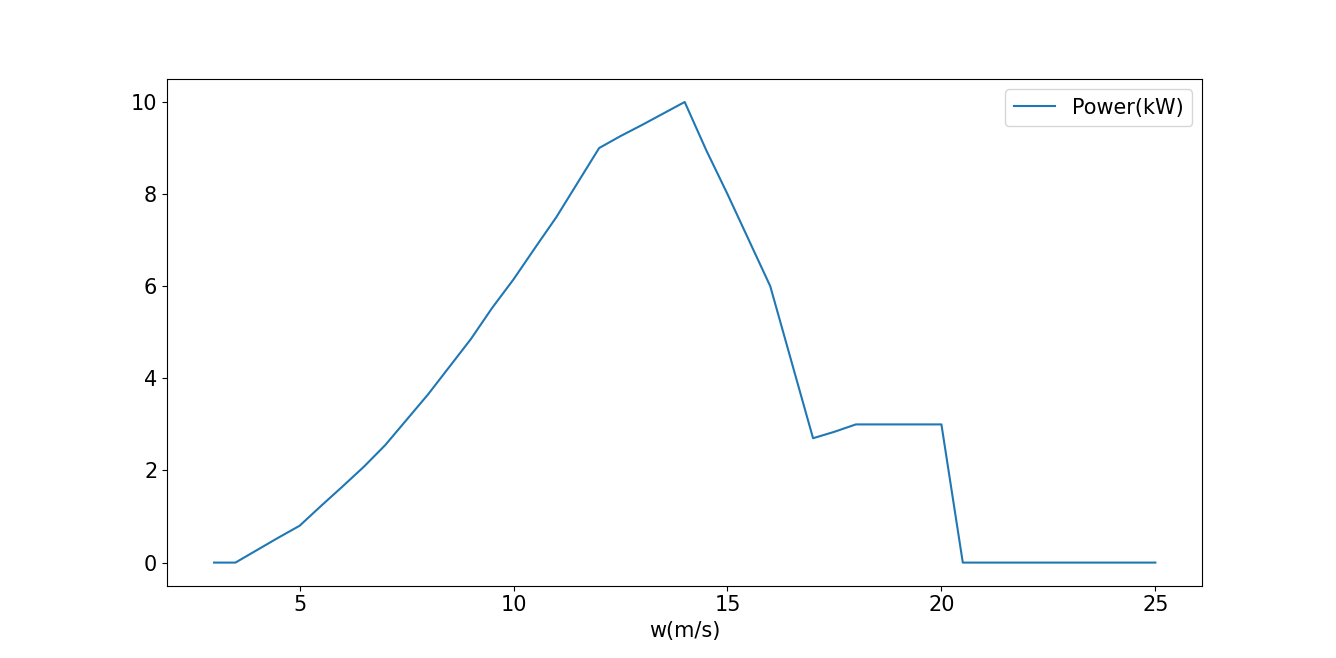
\includegraphics[width=0.8\textwidth]{../img/bergey.png}
		\caption{Curva original}\label{fig:bergey}
	\end{subfigure}
	\\ \vspace{0.5cm}
	\begin{subfigure}[b]{\textwidth}
		\centering
		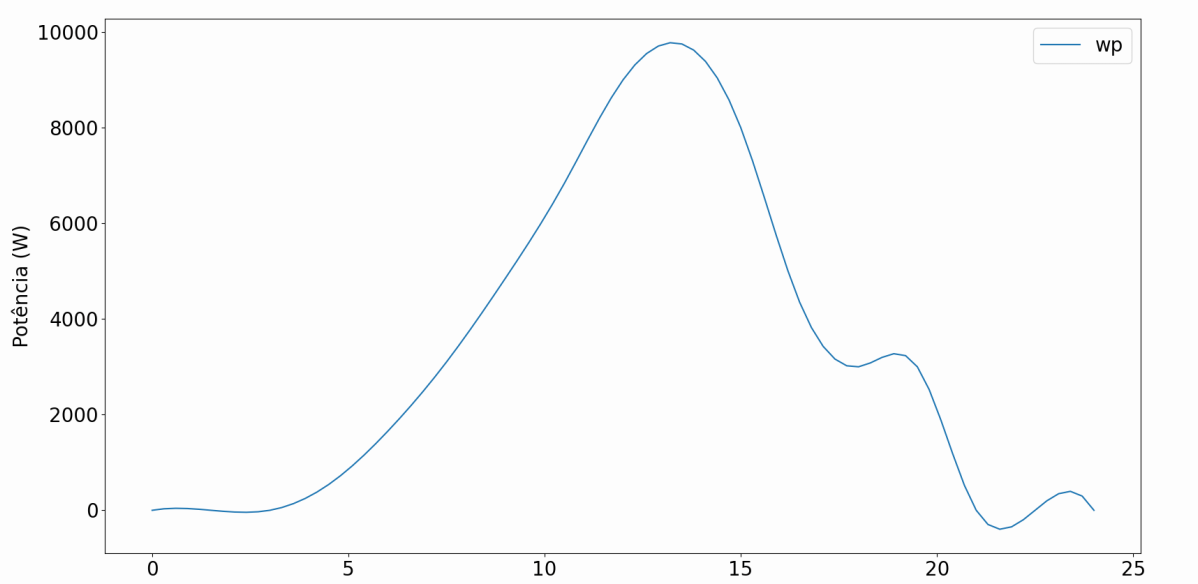
\includegraphics[width=0.8\textwidth]{../img/bergey_corr.png}
		\caption{Curva interpolada}\label{fig:bergey_corr}
	\end{subfigure}
	\caption{Curva de potência do aerogerador \emph{Bergey Excel-10}. Fonte: própria.}\label{fig:wind:power}
\end{figure}
